\documentclass[ucs,9pt]{beamer}

% Copyright 2004 by Till Tantau <tantau@users.sourceforge.net>.
%
% In principle, this file can be redistributed and/or modified under
% the terms of the GNU Public License, version 2.
%
% However, this file is supposed to be a template to be modified
% for your own needs. For this reason, if you use this file as a
% template and not specifically distribute it as part of a another
% package/program, I grant the extra permission to freely copy and
% modify this file as you see fit and even to delete this copyright
% notice.
%
% Modified by Tobias G. Pfeiffer <tobias.pfeiffer@math.fu-berlin.de>
% to show usage of some features specific to the FU Berlin template.

% remove this line and the "ucs" option to the documentclass when your editor is not utf8-capable
\usepackage[utf8x]{inputenc}    % to make utf-8 input possible
\usepackage[english,german]{babel}     % hyphenation etc., alternatively use 'german' as parameter
\usepackage{hyperref}

% Template for talks using the Corporate Design of the Freie Universitaet
%   Berlin, created following the guidelines on www.fu-berlin.de/cd by
%   Tobias G. Pfeiffer, <tobias.pfeiffer@math.fu-berlin.de>
% This file can be redistributed and/or modified in any way you like.
%   If you feel you have done significant improvements to this template,
%   please consider providing your modified version to
%   https://www.mi.fu-berlin.de/w/Mi/BeamerTemplateCorporateDesign

\usepackage{amsmath,dsfont,listings}

%%% FU logo
% small version for upper right corner of normal pages
\pgfdeclareimage[height=0.9cm]{university-logo}{FULogo_RGB}
\logo{\pgfuseimage{university-logo}}
% large version for upper right corner of title page
\pgfdeclareimage[height=1.085cm]{big-university-logo}{FULogo_RGB}
\newcommand{\titleimage}[1]{\pgfdeclareimage[height=2.92cm]{title-image}{#1}}
\titlegraphic{\pgfuseimage{title-image}}
%%% end FU logo

% NOTE: 1cm = 0.393 in = 28.346 pt;    1 pt = 1/72 in = 0.0352 cm
\setbeamersize{text margin right=3.5mm, text margin left=7.5mm}  % text margin

% colors to be used
\definecolor{text-grey}{rgb}{0.45, 0.45, 0.45} % grey text on white background
\definecolor{bg-grey}{rgb}{0.66, 0.65, 0.60} % grey background (for white text)
\definecolor{fu-blue}{RGB}{0, 51, 102} % blue text
\definecolor{fu-green}{RGB}{153, 204, 0} % green text
\definecolor{fu-red}{RGB}{204, 0, 0} % red text (used by \alert)

% switch off the sidebars
% TODO: loading \useoutertheme{sidebar} (which is maybe wanted) also inserts
%   a sidebar on title page (unwanted), also indents the page title (unwanted?),
%   and duplicates the navigation symbols (unwanted)
\setbeamersize{sidebar width left=0cm, sidebar width right=0mm}
\setbeamertemplate{sidebar right}{}
\setbeamertemplate{sidebar left}{}
%    XOR
% \useoutertheme{sidebar}

% frame title
% is truncated before logo and splits on two lines
% if neccessary (or manually using \\)
\setbeamertemplate{frametitle}{%
    \vskip-30pt \color{text-grey}\large%
    \begin{minipage}[b][23pt]{80.5mm}%
    \flushleft\insertframetitle%
    \end{minipage}%
}

%%% title page
% TODO: get rid of the navigation symbols on the title page.
%   actually, \frame[plain] *should* remove them...
\setbeamertemplate{title page}{
% upper right: FU logo
\vskip2pt\hfill\pgfuseimage{big-university-logo} \\
\vskip6pt\hskip3pt
% title image of the presentation
\begin{minipage}{11.6cm}
\hspace{-1mm}\inserttitlegraphic
\end{minipage}

% set the title and the author
\vskip14pt
\parbox[top][1.35cm][c]{11cm}{\color{text-grey}\inserttitle \\ \small \insertsubtitle}
\vskip11pt
\parbox[top][1.35cm][c]{11cm}{\small \insertauthor \\ \insertinstitute \\[3mm] \insertdate}
}
%%% end title page

%%% colors
\usecolortheme{lily}
\setbeamercolor*{normal text}{fg=black,bg=white}
\setbeamercolor*{alerted text}{fg=fu-red}
\setbeamercolor*{example text}{fg=fu-green}
\setbeamercolor*{structure}{fg=fu-blue}

\setbeamercolor*{block title}{fg=white,bg=black!50}
\setbeamercolor*{block title alerted}{fg=white,bg=black!50}
\setbeamercolor*{block title example}{fg=white,bg=black!50}

\setbeamercolor*{block body}{bg=black!10}
\setbeamercolor*{block body alerted}{bg=black!10}
\setbeamercolor*{block body example}{bg=black!10}

\setbeamercolor{bibliography entry author}{fg=fu-blue}
% TODO: this doesn't work at all:
\setbeamercolor{bibliography entry journal}{fg=text-grey}

\setbeamercolor{item}{fg=fu-blue}
\setbeamercolor{navigation symbols}{fg=text-grey,bg=bg-grey}
%%% end colors

%%% headline
\setbeamertemplate{headline}{
\vskip4pt\hfill\insertlogo\hspace{3.5mm} % logo on the right

\vskip6pt\color{fu-blue}\rule{\textwidth}{0.4pt} % horizontal line
}
%%% end headline

%%% footline
\newcommand{\footlinetext}{\insertshortinstitute, \insertshorttitle, \insertshortdate}
\setbeamertemplate{footline}{
\vskip5pt\color{fu-blue}\rule{\textwidth}{0.4pt}\\ % horizontal line
\vskip2pt
\makebox[123mm]{\hspace{7.5mm}
\color{fu-blue}\footlinetext
\hfill \raisebox{-1pt}{\usebeamertemplate***{navigation symbols}}
\hfill \insertframenumber}
\vskip4pt
}
%%% end footline

%%% settings for listings package
\lstset{extendedchars=true, showstringspaces=false, basicstyle=\footnotesize\sffamily, tabsize=2, breaklines=true, breakindent=10pt, frame=l, columns=fullflexible}
\lstset{language=Java} % this sets the syntax highlighting
\lstset{mathescape=true} % this switches on $...$ substitution in code
% enables UTF-8 in source code:
\lstset{literate={ä}{{\"a}}1 {ö}{{\"o}}1 {ü}{{\"u}}1 {Ä}{{\"A}}1 {Ö}{{\"O}}1 {Ü}{{\"U}}1 {ß}{\ss}1}
%%% end listings  % THIS is the line that includes the FU template!

\usepackage{arev,t1enc} % looks nicer than the standard sans-serif font
% if you experience problems, comment out the line above and change
% the documentclass option "9pt" to "10pt"

% image to be shown on the title page (without file extension, should be pdf or png)
\titleimage{fu_500}

\newcommand{\email}[1]{\href{mailto:#1}{#1}}

\title{SWP Übersetzerbau im SS 13}
\subtitle{Einführung und Organisatorisches}
\author{Till~Zoppke \and Maximilian~Konzack \and Yves~Müller}
\institute[FU Berlin]{Freie Universität Berlin}

\date{Auftaktveranstaltung am 13.~April 2013}


% you can redefine the text shown in the footline. use a combination of
% \insertshortauthor, \insertshortinstitute, \insertshorttitle, \insertshortdate, ...
\renewcommand{\footlinetext}{\insertshortinstitute, \insertshorttitle, \insertshortdate}

% Delete this, if you do not want the table of contents to pop up at
% the beginning of each subsection:
%\AtBeginSubsection[]
%{
%  \begin{frame}<beamer>{Outline}
%    \tableofcontents[currentsection,currentsubsection]
%  \end{frame}
%}

\begin{document}

\begin{frame}[plain]
  \titlepage
\end{frame}

\begin{frame}{Übersicht}
  \tableofcontents
\end{frame}

\section{Projektidee}
\begin{frame}
  \frametitle{Entwicklung eines Compilers im Team}
  \begin{center}
    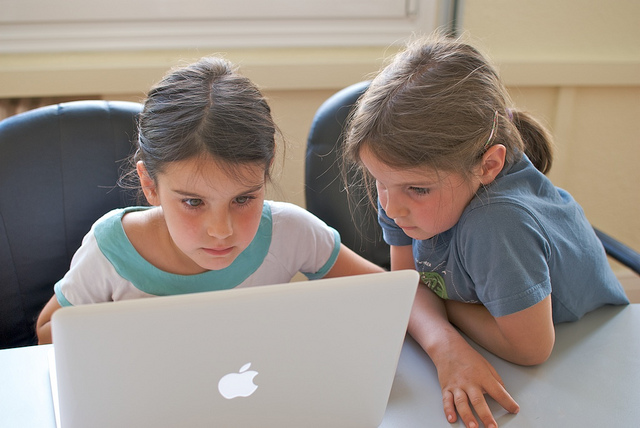
\includegraphics[width=0.7\textwidth]{pair_prog}
  \end{center}
\end{frame}
\begin{frame}
  \frametitle{Modularer Compiler}
  \begin{block}{Idee}
    \begin{itemize}
      \item Implementierung eines Übersetzers
      \item soll im Rahmen der Übersetzerbau genutzt werden können
      \item Quellsprache ist imperativ und statisch typisiert
    \end{itemize}
  \end{block}

  \begin{columns}
    \begin{column}{0.3\textwidth}
  \begin{center}
    
\includegraphics[height=3cm]{java_duke}
  \end{center}
\end{column}
    \begin{column}{0.7\textwidth}
  \begin{block}{Ziele}
      \begin{description}
          \item[modular] Abgrenzung gegenüber anderen Modulen
          \item[einfach] Verwendbarkeit mit anderen Komponenten
          \item[getestet] Black- und Whiteboxtests
          \item[dokumentiert] im Quellcode und als Text
      \end{description}
  \end{block}
\end{column}
  \end{columns}
\end{frame}

\begin{frame}
    \frametitle{Veranschaulichung der zu erstellenden Artefakte}
    \begin{center}
        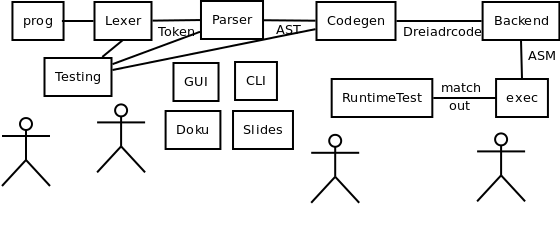
\includegraphics[width=0.9\textwidth]{pipeline}
    \end{center}
    \begin{itemize}
        \item bekannte Aufteilung in Front- und Backend
        \item Projektmanagement bezogene Artefakte
            \begin{enumerate}
                \item Präsentationen
                \item Dokumentation
            \end{enumerate}
        \item Visualisierung als GUI und/oder Commandline Interface von
            \begin{enumerate}
                \item abstrakter Syntax (AST) als ASCII, xml, SVG, \dots
                \item drei Adresscode als Text, Tripel-, Quadrupeldarstellung,
                    \dots
                \item anderen Ergebnissen: Interpreter, Debugger, \dots
            \end{enumerate}
    \end{itemize}
\end{frame}

\section{Einteilung in Gruppen}
\begin{frame}
    \frametitle{Aufteilung in Gruppen}
    \begin{block}{Gruppengröße}
        \begin{itemize}
            \item $\approx 25$ Teilnehmer im KVV
            \item 2 Gruppen mit $\approx 12,5$ Teilnehmer
        \end{itemize}
    \end{block}
    \begin{block}{Organisation}
        \begin{itemize}
            \item grundsätzlich frei gestellt
            \item zwei unterschiedlichen Zielcode:
                \begin{enumerate}
                    \item Java Bytecode
                    \item LLVM, GNU Assembler, \dots
                \end{enumerate}
            \item jedoch legen wir Wert auf:
                \begin{enumerate}
                    \item Inkrementelle Software Entwicklung
                    \item Implementierung
                    \item Interface Spezifikation
                    \item Automatisierung der verschiedenen Tests
                    \item Visualisierung der Ergebnisse über Commandline, GUI,
                        \dots
                \end{enumerate}
        \end{itemize}
    \end{block}
\end{frame}

\section{Organisatorisches}
\subsection{Treffen}
\begin{frame}
  \frametitle{Projekttreffen}
  \begin{block}{Treffen aller Teilnehmer}
    \begin{itemize}
      \item alle zwei Wochen
      \item donnerstags von 14 bis 16 Uhr c.t. im SR~049
      \item bei zu vielen Fehlterminen wird Anwesenheitspflicht eingeführt!
      \item von jedem Teilnehmer wird erwartet mindestens \emph{1x} zu
          präsentieren
    \end{itemize}
  \end{block}
  $\Rightarrow$ andere Woche für Statusbericht und projektinterne Treffen vormerken!

  \begin{block}{Zweck der Projekttreffen}
    \begin{enumerate}
        \item Arbeitsfortschritt
        \item Wissensaustausch
        \item Projektmanagement
        \item Visualisierung der Ergebnisse
        \item Probleme, Fragen, Diskussion, \dots
    \end{enumerate}
  \end{block}
\end{frame}

\begin{frame}
    \frametitle{Vorgaben zu den Präsentationen}
    \begin{block}{Allgemeines}
        \begin{itemize}
            \item Dauer eines Vortrags $\approx$ 15~Minuten
                \begin{itemize}
                    \item 10 Minuten davon für Präsentation
                    \item 5 Minute für Fragen vorsehen
                \end{itemize}
            \item im Zweifel weniger Folien sind besser!
        \end{itemize}
    \end{block}
    \begin{columns}
        \begin{column}{0.5\textwidth}
            \begin{block}{Präsentation zum Meilenstein}
               Fokus auf Projektalltag:
               \begin{enumerate}
                   \item Projektstruktur
                   \item Status zum Meilenstein
                   \item Aufgabenverteilung
                   \item Projektmanagement
                   \item Demonstration des Compilers
                   \item \dots
               \end{enumerate}
            \end{block}
        \end{column}
        \begin{column}{0.5\textwidth}
            \begin{block}{Fachvortrag}
               Fokus auf Wissensaustausch. Mögliche Themen:
               \begin{enumerate}
                   \item Aufbau und Struktur von Java Bytecode
                   \item git (Branch und Merge Strategien, Issues, \dots)
                   \item Design Patterns (Visitor, Interpreter,
                       Factory, \dots)
                   \item JUnit
               \end{enumerate}
            \end{block}
        \end{column}
    \end{columns}
\end{frame}

\begin{frame}
    \frametitle{Statusbericht über Meilenstein}
    \begin{itemize}
        \item kurzer Status Strukturierung des Meilensteins
        \item wenn \emph{kein Projekttreffen} ist
    \end{itemize}
        \begin{block}{Was wollen wir sehen?}
            mind. 1 Punkt aus folgenden:
            \begin{itemize}
                \item Offene und abgeschlossene Tickets/Issues
                \item To-Do-Liste
                \item Projektverlaufsplan
                \item Mündlicher Bericht
                \item \dots
            \end{itemize}
        \end{block}
        \begin{block}{Was \emph{nicht}?}
            alles was im Vortrag zum Meilenstein gehört
        \end{block}
\end{frame}

\subsection{Bürozeiten der Betreuer}
\begin{frame}
    \frametitle{Bürozeiten der Betreuer}
    Betreuer des Softwareprojekts sind
    \begin{enumerate}
        \item Till Zoppke Email:~\email{zoppke@zedat.fu-berlin.de}
        \item Maximilian Konzack Email:~\email{maximilian.konzack@fu-berlin.de}
        \item Yves Müller Email:~\email{yves.mueller@fu-berlin.de}
    \end{enumerate}
    \begin{block}{Wo und wann?}
        Donnerstags 16 bis 18 Uhr im SR~158
    \end{block}
    \begin{block}{Wann zu nutzen?}
        bei
        \begin{itemize}
            \item Problemen im Team
            \item Unklarheiten
            \item Fragen
            \item Anregungen
            \item \dots
        \end{itemize}
    \end{block}
\end{frame}

\subsection{Bewertung}
\begin{frame}
    \frametitle{Bewertungsschema}
    umfasst
    \begin{enumerate}
        \item Quellcode
        \item Dokumentation
        \item Präsentationen
        \item Abschluss
    \end{enumerate} bezüglich der Meilensteine
    \begin{block}{Meilensteine}
        \begin{description}
            \item[M1] Arithmetik
            \item[M2] \texttt{print} Anweisung und Verzweigungen
            \item[M3] Schleifen und Arrays
        \end{description}
    \end{block}
\end{frame}

\subsection{Repositories}
\begin{frame}
    \frametitle{Verwaltung des SWPs auf GitHub}
    GitHub Organisation für das SWP:
    \url{https://github.com/swp-uebersetzerbau-ss13}
  \begin{columns}
    \begin{column}{0.5\textwidth}
  \begin{center}
    
\includegraphics[height=2cm]{githuboctacat}
  \end{center}
\end{column}
    \begin{column}{0.5\textwidth}
  \begin{block}{Repositories}
      \begin{enumerate}
          \item Ein \emph{allgemeines Repository} für projektübergreifende
              \begin{itemize}
                  \item Dokumentation
                  \item Beispiele
                  \item Tests
                  \item Interfaces
              \end{itemize}
          \item \emph{jede} Gruppe erhält eigenes Repository für ihre
              Implementierung
      \end{enumerate}
  \end{block}
\end{column}
  \end{columns}
\end{frame}

\section{Git Primer}
\begin{frame}
    \frametitle{Einführung in git}
  \begin{columns}
    \begin{column}{0.3\textwidth}
  \begin{center}
    
\includegraphics[width=3cm]{git_logo}
  \end{center}
\end{column}
    \begin{column}{0.7\textwidth}
  \begin{block}{Was ist git?}
      \begin{enumerate}
          \item Versionsverwaltung von Dateien, insbesondere für Quellcode
          \item freie Software
          \item geeignet für kleine bis große Projekte
          \item kann nur nur lokal (auf einem Rechner) oder stark verteilt
              genutzt werden
          \item viele große Open Source Projekte nutzen git
      \end{enumerate}
  \end{block}
\end{column}
  \end{columns}
  \end{frame}

  \begin{frame}[fragile]
    \frametitle{Wichtige Befehle für die Arbeit mit git}
    \begin{enumerate}
        \item Lokale Kopie vom Repository anlegen:
            \begin{verbatim}
            $ git clone <repo>
            \end{verbatim}
        \item Revision ansehen:
            \begin{verbatim}
            $ git show <rev number>
            \end{verbatim}
        \item Lokalen Veränderungen (noch ohne commit) ansehen:
            \begin{verbatim}
            $ git status
            \end{verbatim}
        \item Commit auf lokalem Repo:
            \begin{verbatim}
            $ git commit -m "message" -a|<file>|<dir>
            \end{verbatim}
        \item Veränderungen vom remote Repo ziehen:
            \begin{verbatim}
            $ git pull origin <branch>
            \end{verbatim}
        \item Eigene Commits auf remote Repo hoch laden:
            \begin{verbatim}
            $ git push origin <branch>
            \end{verbatim}
    \end{enumerate}
\end{frame}

\begin{frame}[fragile]
    \frametitle{Befehle zur Verwaltung von Branches}
    \begin{enumerate}
        \item Erstelle einen neuen Branch (und wechsle zu ihm):
            \begin{verbatim}
            $ git checkout -b <branch>
            \end{verbatim}
        \item Zeige alle verfügbaren Branches:
            \begin{verbatim}
            $ git branch -a
            \end{verbatim}
        \item Wechsele vom aktuellen Branch zu angegeben:
            \begin{verbatim}
            $ git checkout <branch>
            \end{verbatim}
        \item Merge von aktuellen Branch mit angegeben:
            \begin{verbatim}
            $ git merge <branch>
            \end{verbatim}
    \end{enumerate}
\end{frame}

\section{Ende}
\begin{frame}
  \frametitle{Ende}
  \begin{center}
    \Huge
    Danke für die Aufmerksamkeit.\\[1em]
    
\includegraphics[height=5cm]{compilers}
    \ 
  \end{center}
\end{frame}

\begin{frame}
    \frametitle{To Dos bis zum nächsten mal}
    \begin{center}
        \begin{enumerate}
            \item git Repo auschecken
            \item Projekteinfindung
            \item Quellsprache verstehen
            \item Projektstruktur festlegen
            \item Meilstein strukturieren
            \item Entwurf von Interfaces
            \item \dots
        \end{enumerate}
    \end{center}
\end{frame}

% All of the following is optional and typically not needed. 
\appendix
\section*{\appendixname}

\begin{frame}
  \frametitle{Literatur}
    
  \begin{thebibliography}{10}
    
  \beamertemplatebookbibitems
  % Start with overview books.

  
  \bibitem[AUS08]{Aho08}
    Alfred~V. Aho, Jeffrey Ullman, and Ravi Sethi.
    \newblock {\em Compiler: {P}rinzipien, {T}echniken und {W}erkzeuge}.
    \newblock Pearson Studium, 2. edition, 2008.


  \bibitem[Fin]{FindBugsWeb}
    {F}ind{B}ugs -- {F}ind {B}ugs in {J}ava {P}rograms.
    \newblock {\url{http://findbugs.sourceforge.net/}}.
  
   \bibitem[GitHub]{GitHubWeb}
    {G}it{H}ub
    \newblock {\url{https://github.com/}}.

   \bibitem[GitRef]{GitRefWeb}
       {G}it {R}eference
    \newblock {\url{http://gitref.org/}}.

   \bibitem[GitNotes]{GitNotesWeb}
       {S}ome {N}otes on {G}it
    \newblock {\url{http://java.dzone.com/articles/some-notes-git}}.

    \bibitem[Sco09]{Scott09}
      Michael~Lee Scott.
      \newblock {\em Programming language pragmatics}.
      \newblock Morgan Kaufmann Publishers, 3. edition, 2009.
    
  \end{thebibliography}
\end{frame}

\end{document}
